% !TeX root = writeup.tex 

\section{Proofs of Main Theorems}  \label{sec:main_thm_proofs}

We are now ready to present and prove theorems that characterize the selection rates under fairness constraints, namely $\dempar$ and $\eqop$. These characterizations are crucial for proving the results in Section \ref{sec:results}. Our computations also generalize readily to other linear constraints, in a way that will become clear in Section \ref{sec:eqop_proof}.

\begin{figure*}[t]

\centering
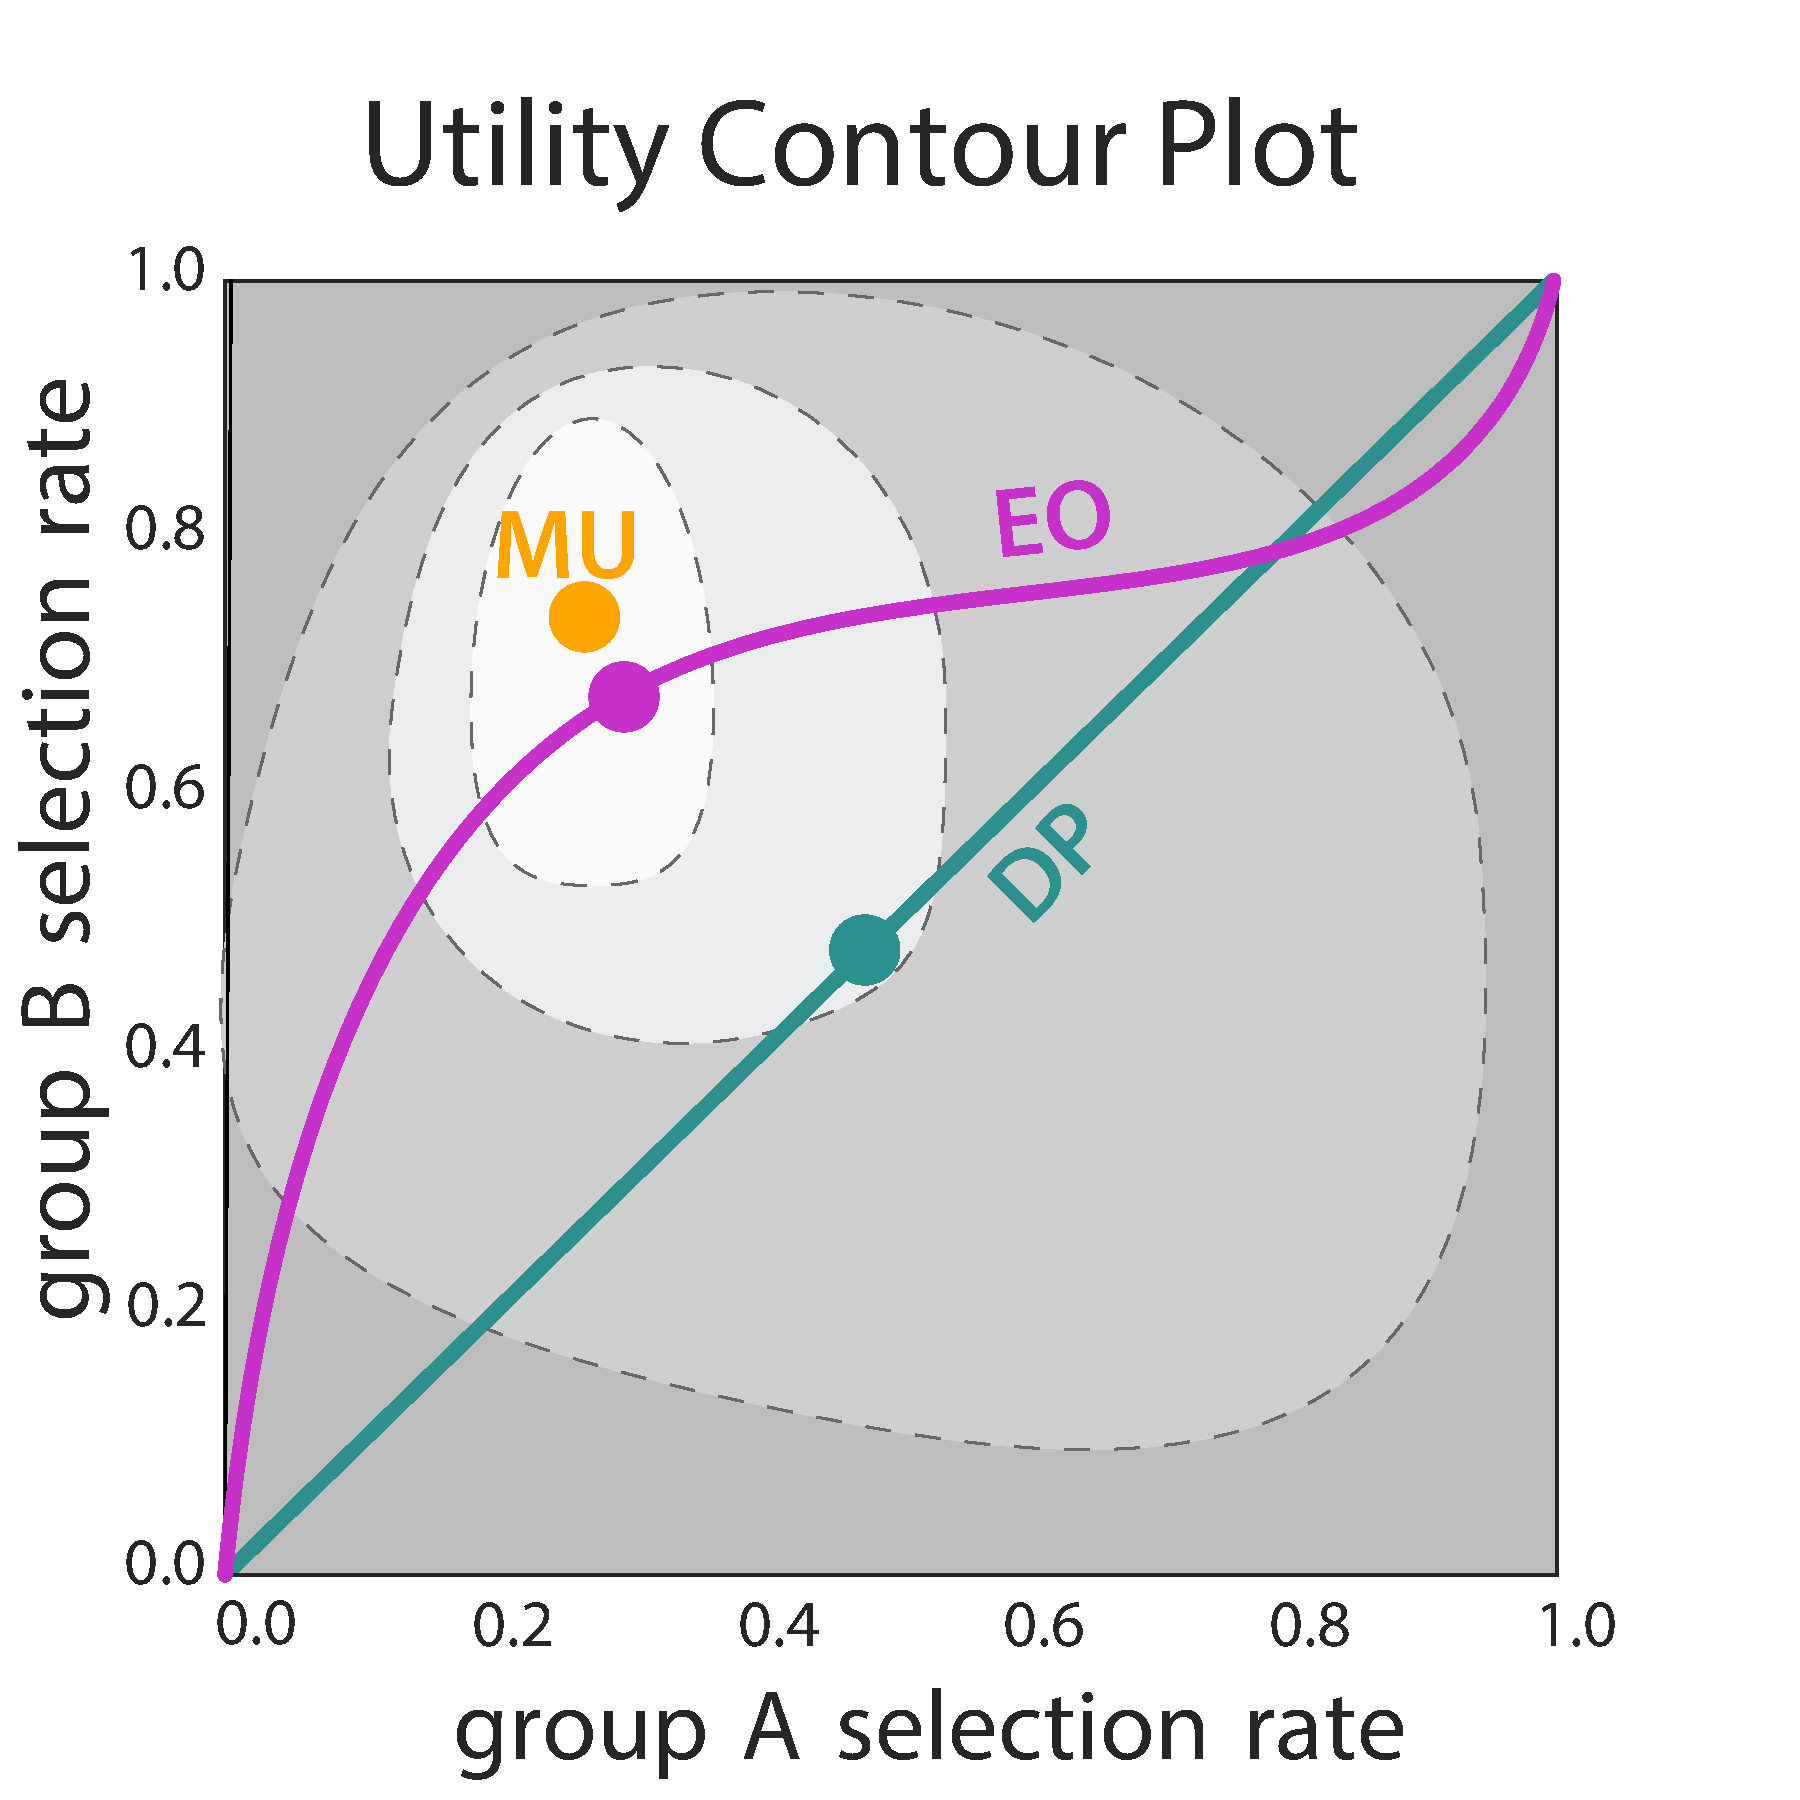
\includegraphics[width=.4\textwidth]{figures/contour_cartoon.pdf}

\caption{ \label{fig:contour} Considering the utility as a function of selection rates, fairness constraints correspond to restricting the optimization to one-dimensional curves. The $\dempar$ (DP) constraint is a straight line with slope $1$, while the $\eqop$ (EO) constraint is a curve given by the graph of $\transfer$. 
%The $\maxprof$ (MU) solution is given as a single dot which corresponds to the heighest point on the utility contour plot.  
The derivatives considered throughout Section~\ref{sec:main_thm_proofs} are taken with respect to the selection rate $\accratea$ (horizontal axis); projecting the EO and DP constraint curves to the horizontal axis recovers concave utility curves such as those shown in the lower panel of Figure~\ref{fig:outcome_util_curves} (where $\maxprof$ in is represented by a horizontal line through the MU optimal solution). }

\end{figure*}

	\subsection{A Characterization Theorem for $\dempar$}\label{sec:dem_par_proof}
		In this section, we provide a theorem that gives an explicit characterization for the range of selection rates $\accratea$ for $\popa$ when the bank loans according to $\dempar$. 
		%
		Observe that the $\dempar$ objective corresponds to solving the following linear program:
		%
		\begin{eqnarray*}\label{eq:hard_const_dempar}
		\max_{\pol = (\pola,\polb) \in [0,1]^{2\maxscore}}\Util(\pol) \quad \subto \quad \langle \dista, \pola \rangle = \langle \distb, \polb \rangle \:.
		\end{eqnarray*}
		Let us introduce the auxiliary variable $\accrate := \langle \dista, \pola \rangle = \langle \distb, \polb \rangle$ corresponding to the selection rate which is held constant across groups, so that all feasible solutions lie on the green DP line in Figure~\ref{fig:contour}. We can then express the following equivalent linear program:
		\begin{eqnarray*}\label{eq:hard_const_dempar_subst}
		\max_{\pol = (\pola,\polb) \in [0,1]^{2\maxscore},\accrate \in [0,1]}\Util(\pol) \quad \subto \quad \accrate = \langle \distj, \polj \rangle,~ \popj \in \{\popa,\popb\}\:.
		\end{eqnarray*}
		This is equivalent because, for a given $\accrate$, Proposition \ref{prop:opt_threshold_fair} says that the utility maximizing policies are of the form $\polj = \ratef_{\distj}^{-1}(\accrate)$. We now prove this:
		
		\begin{proof}[Proof of Proposition~\ref{prop:opt_threshold_fair} for $\dempar$] 
				Noting that $\ratef_{\distj}(\polj) = \langle \distj , \polj \rangle$, we see that, by Lemma~\ref{lem:optimal_best}, under the special case where $\boldv(x) = \util(x)$ and $\boldw(x) = 1$, the optimal solution $(\pola^*(\accrate),\polb^*(\accrate))$ for fixed $\ratef_{\dista}(\pola) = \ratef_{\distb}(\polb) = \accrate$ can be chosen to coincide with the threshold policies. Optimizing over $\accrate$, the global optimal must coincide with thresholds. 
				
		\end{proof}
		
		
			
		
		Hence, any optimal policy is equivalent to the threshold policy $\pol = (\ratef_{\dista}^{-1}(\accrate),\ratef_{\distb}^{-1}(\accrate))$, where $\accrate$ solves the following optimization:
		\begin{eqnarray}\label{eq:hard_const_dempar_accrate}
		\max_{\accrate \in [0,1]}\Util\left(\left(\ratef_{\dista}^{-1}(\accrate),\ratef_{\distb}^{-1}(\accrate)\right)\right) \:.
		\end{eqnarray}
		We shall show that the above expression is in fact a \emph{concave} function in $\accrate$, and hence the set of optimal selection rates can be characterized by first order conditions. This is presented formally in the following theorem:

	\begin{thm}[Selection rates for $\dempar$]\label{thm:dem_par_selection}
	
	The set of optimal selection rates $\accrate^*$ satisfying~\eqref{eq:hard_const_dempar_accrate} forms a continuous interval $[\accrate_{\dempar}^-,\accrate_{\dempar}^+]$, such that for any $\accrate \in [0,1]$, we have
	\begin{eqnarray*}
	\accrate < \accrate_{\dempar}^- &\text{if}& \fraca\util\left(\RCDF\supa(\accrate)\right) + \fracb\util\left(\RCDF\supb(\accrate)\right) > 0\:, \\
	\accrate > \accrate_{\dempar}^+ &\text{if}& \fraca\util\left(\RCDFpl\supa(\accrate) \right)+ \fracb\util\left(\RCDFpl\supb(\accrate)\right) < 0\:. \\
	\end{eqnarray*}
		\end{thm}
		\begin{proof}  Note that we can write 
		\begin{eqnarray*}
		% \Util\left((\pola,\polb)\right)  &= \fraca\langle \util, \dista \circ  \pola \rangle + \fracb\langle \util, \distb \circ  \polb \rangle  \\
		\Util\left(\left(\ratef_{\dista}^{-1}(\accrate),\ratef_{\distb}^{-1}(\accrate)\right)\right)  &= \fraca\langle \util, \dista \circ  \ratef_{\dista}^{-1}(\accrate) \rangle + \fracb\langle \util, \distb \circ  \ratef_{\distb}^{-1}(\accrate) \rangle \:.
		\end{eqnarray*}
		%  \begin{eqnarray*}
		% \Util\left((\pola,\polb)\right)  = \fraca\langle \util, \dista \circ  \pola \rangle + \fracb\langle \util, \distb \circ  \polb \rangle 
		% \end{eqnarray*}

		Since $\util(x)$ is non-decreasing in $x$, Proposition~\ref{prop:beta_concavity} implies that $\beta \mapsto \Util\left(\left(\ratef_{\dista}^{-1}(\accrate),\ratef_{\distb}^{-1}(\accrate)\right)\right)$ is concave in $\accrate$. Hence, all optimal selection rates $\accrate^*$ lie in an interval $[\beta^-,\beta^+]$. To further characterize this interval, let us us compute left- and right-derivatives.
		\begin{eqnarray*}
		\partial_+ \Util\left(\left(\ratef_{\dista}^{-1}(\accrate),\ratef_{\distb}^{-1}(\accrate)\right)\right) &=& 
		\partial_+ \fraca\langle \util, \dista \circ \ratef_{\dista}^{-1}(\accrate) \rangle + \partial_+ \fracb  \langle \util , \distb \circ \ratef_{\distb}^{-1}(\accrate) \rangle\\
		&=& \fraca\langle \util, \partial_+ \left( \dista \circ \ratef_{\dista}^{-1}(\accrate) \right)\rangle + \fracb \langle \util , \partial_+  \left( \distb \circ\ratef_{\distb}^{-1}(\accrate) \right) \rangle\\
		&\overset{\text{Lemma}~\ref{lem:der_comp}}{=}& \fraca\langle \util, \bolde_{\RCDF\supa(\beta)}  \rangle + \fracb \langle \util ,  \bolde_{\RCDF\supb(\beta)}  \rangle\\
		&=& \fraca \util(\RCDF\supa(\beta))  + \fracb \util(\RCDF\supb(\beta))\:.
		\end{eqnarray*}
		The same argument shows that 
		\begin{eqnarray*}
		\partial_- \Util((\ratef_{\dista}^{-1}(\accrate),\ratef_{\distb}^{-1}(\accrate))) = \fraca \util(\RCDFpl\supa(\beta))  + \fracb \util(\RCDFpl\supb(\beta)).	\end{eqnarray*} 
		By concavity of $\Util\left(\left(\ratef_{\dista}^{-1}(\accrate),\ratef_{\distb}^{-1}(\accrate)\right)\right)$, a positive right derivative at $\accrate$ implies that $\accrate <  \accrate^*$ for all $\beta^*$ satisfying~\eqref{eq:hard_const_dempar_accrate}, and similarly, a negative left derivative at $\accrate$ implies that $\accrate >  \accrate^*$ for all $\beta^*$ satisfying ~\eqref{eq:hard_const_dempar_accrate}.
	
		\end{proof}
		
		With a result of the above form, we can now easily prove statements such as that in Corollary \ref{cor:dp_overeager} (see appendix \ref{app:main_results_proofs} for proofs), by fixing a selection rate of interest (e.g. $\beta_0$) and inverting the inequalities in Theorem \ref{thm:dem_par_selection} to find the exact population proportions under which, for example, $\dempar$ results in a higher selection rate than $\beta_0$.

	\subsection{$\eqop$ and General Constraints} \label{sec:eqop_proof}
		Next, we will provide a theorem that gives an explicit characterization for the range of selection rates $\accratea$ for $\popa$ when the bank loans according to $\eqop$. 
		%
		Observe that the $\eqop$ objective corresponds to solving the following linear program:
		\begin{eqnarray}\label{eq:hard_const_eqop}
		\max_{\pol = (\pola,\polb) \in [0,1]^{2\maxscore}}\Util(\pol) \quad \subto \quad \langle \boldwa \circ  \dista, \pola \rangle = \langle \boldwb \circ  \distb, \polb \rangle~,
		\end{eqnarray}
		where $\boldw\supj = \frac{\pb}{\langle \pb, \distj\rangle}$. This problem is similar to the demographic parity optimization in~\eqref{eq:hard_const_dempar_accrate}, except for the fact that the constraint includes the weights. 
		%
		Whereas we parameterized demographic parity solutions in terms of the acceptance rate $\accrate$ in equation~\eqref{eq:hard_const_dempar_accrate}, we will parameterize equation~\eqref{eq:hard_const_eqop} in terms of the true positive rate (TPR), $t:= \langle \boldwa \circ  \dista, \pola \rangle$. Thus,~\eqref{eq:hard_const_eqop} becomes 
		\begin{eqnarray}\label{eq:hard_const_eqop_2}
		\max_{t \in [0,t_{\max}]} \max_{(\pola,\polb) \in [0,1]^{2\maxscore}}\sum_{j \in \pops}\fracj \Util\supj(\polj) \quad \subto \quad \langle \boldwj \circ  \distj, \polj \rangle = t,~\popj\in\pops~,
		\end{eqnarray}
		where $t_{\max} = \min_{\popj \in \pops}\{\langle \distj, \boldwj \rangle\}$ is the largest possible TPR. The magenta EO curve in Figure~\ref{fig:contour} illustrates that feasible solutions to this optimization problem lie on a curve parametrized by $t$.
		Note that the objective function decouples for $\popj \in \pops$ for the inner optimization problem,
		\begin{eqnarray}\label{eq:hard_const_eqop_3}
		\max_{\polj \in [0,1]^{\maxscore}}\sum_{j \in \pops}\fracj \Util\supj(\polj) \quad \subto \quad \langle \boldwj \circ  \distj, \polj \rangle = t\:.
		\end{eqnarray}
		We will now show that all optimal solutions for this inner optimization problem are $\distj$-a.e. equal to a policy in $\Monotone(\distj)$, and thus can be written as $\ratef_{\distj}^{-1}(\accrate\supj)$, depending only on the resulting selection rate.
		
		\begin{proof}[Proof of Proposition~\ref{prop:opt_threshold_fair} for $\eqop$] 
			We apply Lemma~\ref{lem:optimal_best} to the inner optimization in~\eqref{eq:hard_const_eqop_3} with $\boldv(x) = \util(x)$ and $\boldw(x) = \frac{\pb(x)}{\langle \pb, \distj\rangle}$. The claim follows from the assumption that $\util(x)/\pb(x)$ is increasing by optimizing over $t$.
		\end{proof}


		This selection rate $\accrate\supj$ is uniquely determined by the TPR $t$ (proof appears in Appendix~\ref{sec:char_fairness_solns_eqopp}):
		
		\begin{restatable}{lem}{bijectiontpr}
		\label{lem:bijection_tpr_accrate}
Suppose that $\boldw(x) > 0$ for all $x$. Then the function
		\begin{eqnarray*}
		\constfj(\accrate):=	\langle \ratef_{\distj}^{-1}(\accrate),\distj \circ \boldwj \rangle
		\end{eqnarray*}
		is a bijection from $[0,1]$ to $[0,\langle \distj, \boldw \rangle]$. 
		\end{restatable}
		Hence, for any $t \in [0,t_{\max}]$, the mapping from TPR to acceptance rate, $\constfj^{-1}(t)$, is well defined and any solution to~\eqref{eq:hard_const_eqop_3} is $\distj$-a.e. equal to the policy $\ratef_{\distj}^{-1}(\constfj^{-1}(t))$. Thus~\eqref{eq:hard_const_eqop_2} reduces to 
		\begin{eqnarray}\label{eq:hard_const_eqop_accrate}
		%\max_{t \in [0,t_{\max}]} \sum_{j \in \pops}\fracj \Util\supj(\ratef_{\distj}^{-1}(\constfj^{-1}(t)))
		\max_{t \in [0,t_{\max}]} \sum_{j \in \pops}\fracj \Util\supj\left(\ratef_{\distj}^{-1}\left(\constfj^{-1}(t)\right)\right)\:.
		\end{eqnarray}

				


	The above expression parametrizes the optimization problem in terms of a single variable. We shall show that the above expression is in fact a \emph{concave} function in $t$, and hence the set of optimal selection rates can be characterized by first order conditions. This is presented formally in the following theorem:
	%In the appendix, Lemma~\ref{lem:const_to_util_derv} shows that the above expression is in fact a \emph{concave} function in $t$ using the following lemma.
%With this result in hand, we will see that the set of optimal selection rates can be characterized by first order conditions. This is presented formally in the following theorem:
\begin{thm}[Selection rates for $\eqop$]\label{thm:eqop_selection}
	The set of optimal selection rates $\accrate^*$ for group~$\popa$ satsifying~\eqref{eq:hard_const_eqop_2} forms a continuous interval $[\accrate_{\eqop}^-,\accrate_{\eqop}^+]$, such that for any $\accrate \in [0,1]$, we have
	\begin{eqnarray*}
		\accrate < \accrate_{\eqop}^- &\text{if}& \fraca\frac{\util(\RCDF\supa(\accrate))}{\boldwa(\RCDF\supa(\accrate))} + \fracb\frac{\util(\RCDF\supb(\transfer_{\boldw}(\accrate)))}{\boldwb(\RCDF\supb(\transfer_{\boldw}(\accrate)))} > 0 \:,\\
		\accrate > \accrate_{\eqop}^+ &\text{if}& \fraca\frac{\util(\RCDFpl\supa(\accrate))}{\boldwa(\RCDFpl\supa(\accrate))} + \fracb\frac{\util(\RCDFpl\supb(\transfer_{\boldw}(\accrate)))}{\boldwb(\RCDFpl\supb(\transfer_{\boldw}(\accrate)))} < 0 ~.
		\end{eqnarray*}
		Here, $\transfer_{\boldw}(\accrate) := \constf_{\popb,\boldwb}^{-1}(\constf_{\popa,\boldwa}^{-1}(\accrate))$ denotes the (well-defined) map from selection rates $\accratea$ for $\popa$ to the selection rate $\accrateb$ for $\popb$ such that the policies $\pola^* := \ratef_{\dista}^{-1}(\accratea)$ and $\polb^* := \ratef_{\distb}^{-1}(\accrateb)$ satisfy the constraint in~\eqref{eq:hard_const_eqop}. 
		\end{thm}
		%
		\begin{proof}  Starting with the equivalent problem in~\eqref{eq:hard_const_eqop_accrate}, we use the concavity result of Lemma~\ref{lem:const_to_util_derv}. Because the objective function is the positive weighted sum of two concave functions, it is also concave. Hence, all optimal true positive rates $t^*$ lie in an interval $[t^-,t^+]$. To further characterize $[t^-,t^+]$, we can compute left- and right-derivatives, again using the result of Lemma~\ref{lem:const_to_util_derv}.
		\begin{eqnarray*}
		\partial_+ \sum_{j \in \pops}\fracj \Util\supj\left(\ratef_{\distj}^{-1}(\constfj^{-1}(t))\right) &=& 
		\fraca \partial_+\Util\supa\left(\ratef_{\dista}^{-1}(\constfa^{-1}(t))\right) + \fraca \partial_+\Util\supa\left(\ratef_{\dista}^{-1}(\constfa^{-1}(t))\right)\\
		&=& \fraca\frac{\util(\RCDF\supa(\constfa^{-1}(t)))}{\boldwa(\RCDF\supa(\constfa^{-1}(t)))} + \fracb\frac{\util(\RCDF\supb(\constfb^{-1}(t)))}{\boldwb(\RCDF\supb(\constfb^{-1}(t)))}
		\end{eqnarray*}
		The same argument shows that 
		\begin{eqnarray*}
		\partial_- \sum_{j \in \pops}\fracj \Util\supj\left(\ratef_{\distj}^{-1}(\constfj^{-1}(t))\right) = \fraca\frac{\util(\RCDFpl\supa(\constfa^{-1}(t))}{\boldwa(\RCDFpl\supa(\constfa^{-1}(t)))} + \fracb\frac{\util(\RCDFpl\supb(\constfb^{-1}(t)))}{\boldwb(\RCDFpl\supb(\constfb^{-1}(t)))}.	
		\end{eqnarray*} 
		By concavity, a positive right derivative at $t$ implies that $t <  t^*$ for all $t^*$ satisfying~\eqref{eq:hard_const_eqop_accrate}, and similarly, a negative left derivative at $t$ implies that $t >  t^*$ for all $t^*$ satisfying~\eqref{eq:hard_const_eqop_accrate}.

		Finally, by Lemma~\ref{lem:bijection_tpr_accrate}, this interval in $t$ uniquely characterizes an interval of acceptance rates. Thus we translate directly into a statement about the selection rates $\accrate$ for group~$\popa$ by seeing that $\constfa^{-1}(t)=\accrate$ and $\constfb^{-1}(t) = \transfer_{\boldw}(\accrate)$. % where we define $\transfer_{\boldw}(\accrate) := \constf_{\popb,\boldwb}^{-1}(\constf_{\popa,\boldwa}^{-1}(\accrate))$.	
		\end{proof}


		Lastly, we remark that the results derived in this section go through verbatim for any linear constraint of the form $\langle \boldw, \dista \circ \pola \rangle = \langle \boldw, \distb \circ \polb \rangle$, as long as $\util(x)/\boldw(x)$ is increasing in $x$, and $\boldw(x) > 0$. 
		
